%\begin{tikzpicture}[scale=2.2,transform shape]
\begin{tikzpicture}
    \node[anchor=south west,inner sep=0] at (0,0)
        {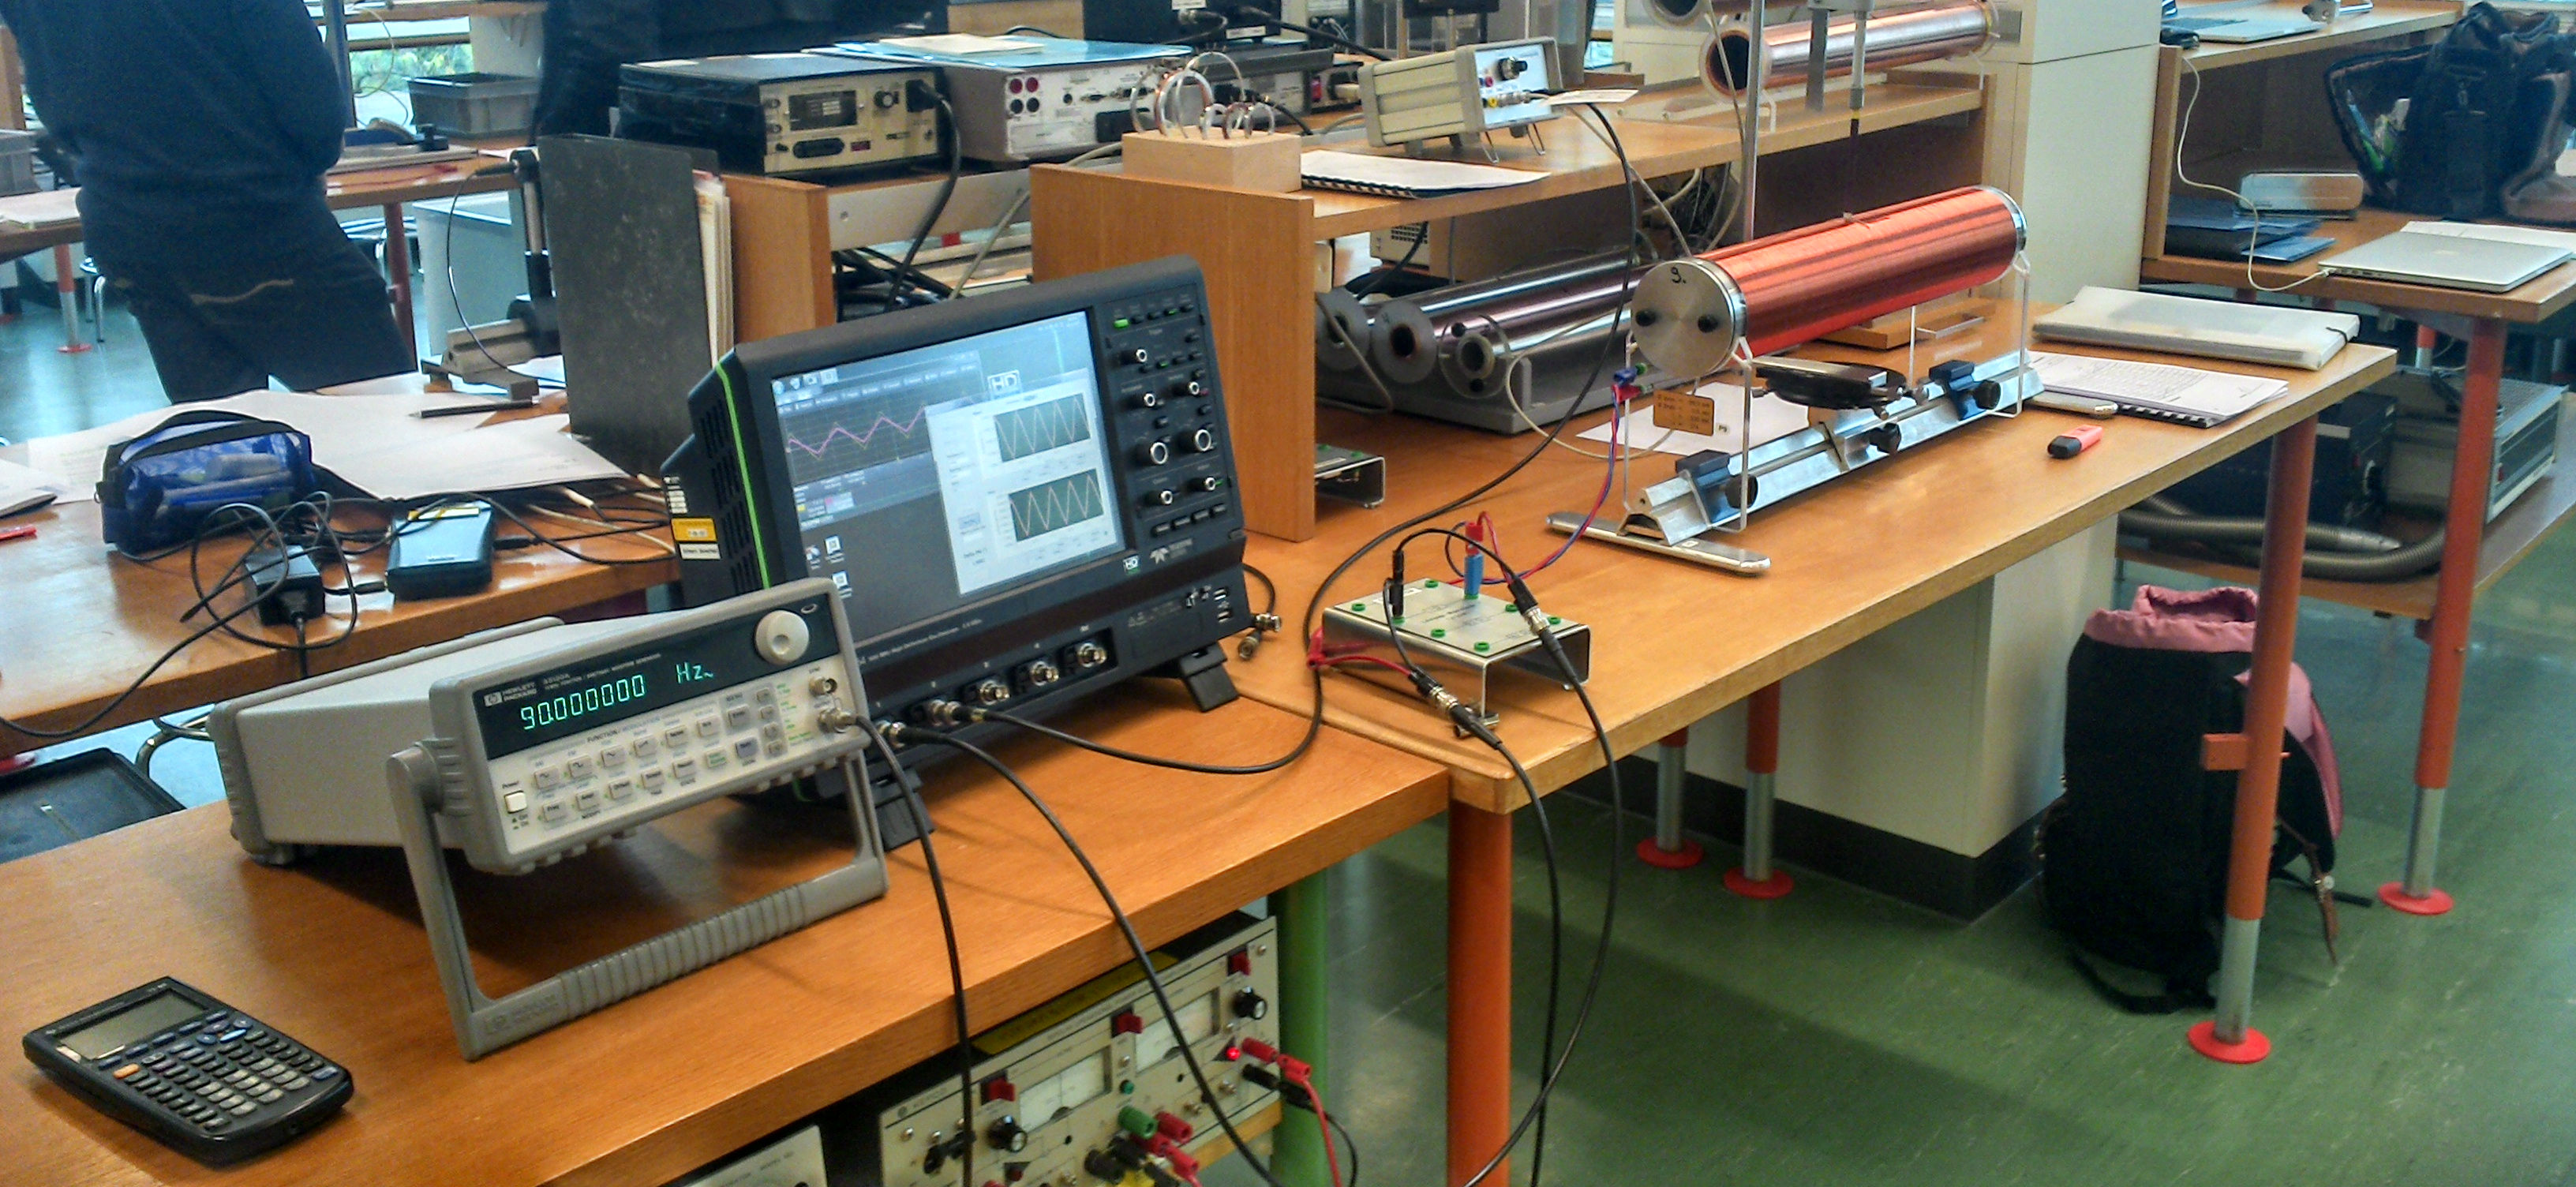
\includegraphics[width=\textwidth]{images/versuchsanordnung-1.jpeg}};

    %\draw[help lines] (0,0) grid (\textwidth,7);

    \fill[black,opacity = 0.6,rounded corners] (1,1) rectangle (1.6,1.8);
    \draw[white,ultra thick,rounded corners] (1,1) rectangle (5,3.45);
    \node at (1.3,1.4) {\huge{\textcolor{white}{1}}};

    \fill[black,opacity = 0.6,rounded corners] (6.4,2) rectangle (7,2.8);
    \draw[green,ultra thick,rounded corners] (4,2) rectangle (7,5);
    \node at (6.7,2.4) {\huge{\textcolor{green}{7}}};

    \fill[black,opacity = 0.6,rounded corners] (8.8,2.5) rectangle (9.4,3.3);
    \draw[yellow,ultra thick,rounded corners] (7.1,2.5) rectangle (9.4,3.6);
    \node at (9.1,2.9) {\huge{\textcolor{yellow}{4}}};

    \fill[white,opacity = 0.6,rounded corners] (11,4) rectangle (11.6,4.8);
    \draw[black,ultra thick,rounded corners] (8.5,4) rectangle (11.6,5.7);
    \node at (11.28,4.4) {\huge{\textcolor{black}{3}}};
\end{tikzpicture}
